\documentclass[border=10pt]{standalone}

\usepackage{tikz}
\usepackage{tikzsymbols}
\usetikzlibrary{calc,patterns,shapes.geometric}

\def\centerarc[#1](#2)(#3:#4:#5){\draw[#1] ($(#2)+({#5*cos(#3)},{#5*sin(#3)})$) arc (#3:#4:#5);}

\begin{document}
	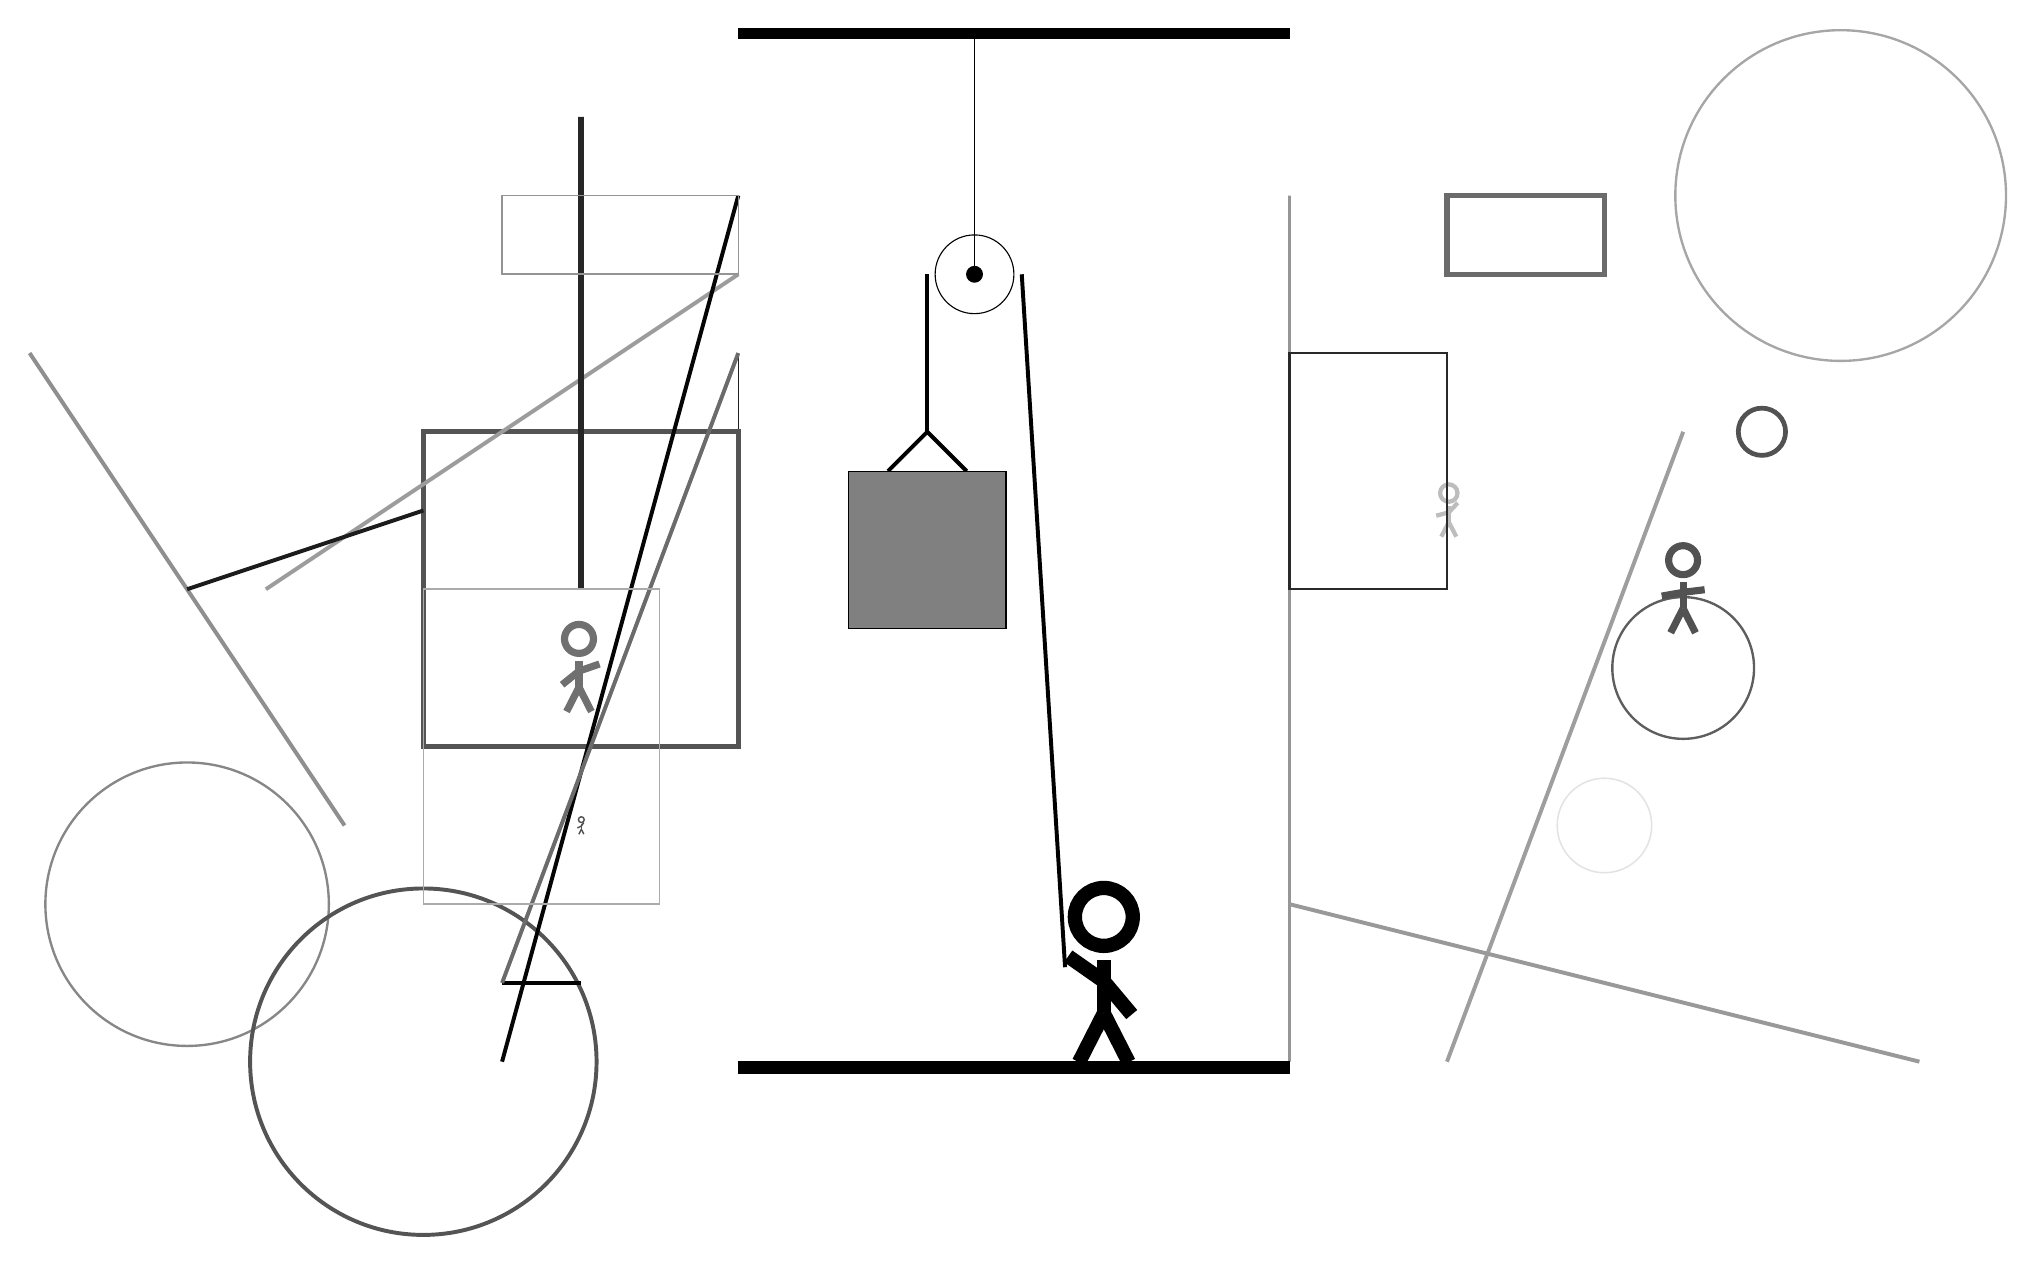
\begin{tikzpicture}
		%%%%% START %%%%%
		
		\draw[fill=black] (-2, 10) rectangle (5, 10.125);
		
		\draw (1, 7) circle (0.5);
		\draw[fill=black] (1, 7) circle (0.1);
		\draw (1, 10) -- (1, 7);
		
		\draw[line width=0.5mm] (-0.1, 4.5) -- (0.4, 5.0) -- (0.9, 4.5);
		\draw[fill=black!50] (-0.6, 4.5) rectangle (1.4, 2.5);
		
		\draw[line width=0.2mm, color=black!88] (-2, 6) rectangle (-2, 1);
		
		\draw [line width=0.2mm, color=black!11](9, 0) circle (0.6);
		\draw [line width=0.3mm, color=black!47](-9, -1) circle (1.8);
		\draw [line width=0.5mm, color=black!67](-6, -3) circle (2.2);
		\draw [line width=0.3mm, color=black!63](10, 2) circle (0.9);
		\draw[line width=0.6mm, color=black!67] (-2, 5) rectangle (-6, 1);
		\draw[line width=0.5mm, color=black!47] (-4, 5) rectangle (-4, 6);
		
		\node[line width=0.5mm, color=black!26] at (7, 4) {\Strichmaxerl[3][15][47]};
		\draw[line width=0.5mm, color=black!39](-2, 7) -- (-8, 3);
		\draw[line width=0.7mm, color=black!85] (-4, 3) rectangle (-4, 9);
		
		\draw [line width=0.3mm, color=black!35](12, 8) circle (2.1);
		
		\draw[line width=0.5mm, color=black!99] (-4, -2) rectangle (-5, -2);
		\draw[line width=0.3mm, color=black!41] (5, 8) rectangle (5, -3);
		\draw[line width=0.5mm, color=black!98](-2, 8) -- (-5, -3);
		\draw [line width=0.6mm, color=black!68](11, 5) circle (0.3);
		\draw[line width=0.5mm, color=black!44](-7, 0) -- (-11, 6);
		\draw[line width=0.2mm, color=black!42] (-2, 7) rectangle (-5, 8);
		\draw[line width=0.7mm, color=black!58] (7, 8) rectangle (9, 7);
		\draw[line width=0.5mm, color=black!58](-2, 6) -- (-5, -2);
		
		\draw[line width=0.5mm, color=black!38](10, 5) -- (7, -3);
		\node[line width=0.2mm, color=black!68] at (10, 3) {\Strichmaxerl[5][10][7]};
		
		\draw[line width=0.5mm, color=black!89](-6, 4) -- (-9, 3);
		
		\node[line width=0.7mm, color=black!56] at (-4, 2) {\Strichmaxerl[5][39][19]};
		\draw[line width=0.2mm, color=black!33] (-3, 3) rectangle (-6, -1);
		\node[line width=0.5mm, color=black!68] at (-4, 0) {\Strichmaxerl[1][25][56]};
		
		\draw[line width=0.5mm, color=black!40](5, -1) -- (13, -3);
		
		\draw[line width=0.3mm, color=black!84] (5, 6) rectangle (7, 3);
		
		\draw[line width=0.5mm] (0.4, 7) -- (0.4, 5.0);
		\centerarc[line width=0.5mm](1, 7)(0:180:0.6);
		\draw[line width=0.5mm](1.6, 7) -- (2.15, -1.8);
		
		\node at (2.6, -1.9) {\Strichmaxerl[10][-35][-50]};
		
		\draw[fill=black] (-2, -3) rectangle (5, -3.15);
		
		%%%%% END %%%%%
	\end{tikzpicture}
\end{document}